
\documentclass[letterpaper,12pt]{article}
\usepackage[hmargin=1in,bmargin=1.5in,tmargin=1.2in]{geometry}
\usepackage{Sweave}
\usepackage{color}
\usepackage{booktabs}
\usepackage{colortbl}
\usepackage{dcolumn}
\usepackage{multirow}
\usepackage{rotating}
\usepackage{tabularx}

\usepackage{tikz}
\usetikzlibrary{calc}
\pgfdeclarelayer{background}
\pgfdeclarelayer{foreground}
\pgfsetlayers{background,main,foreground}\definecolor{colorM1}{RGB}{241,235,230}
 \definecolor{colorM2}{RGB}{211,189,168}
 \definecolor{colorM3}{RGB}{184,152,124}
 \definecolor{colorM4}{RGB}{124,108,92}
 \definecolor{colorM5}{RGB}{88,48,8}
 \definecolor{colorA1}{RGB}{195,229,208}
 \definecolor{colorA2}{RGB}{164,229,188}
 \definecolor{colorA3}{RGB}{86,156,112}
 \definecolor{colorA4}{RGB}{67,90,75}
 \definecolor{colorA5}{RGB}{6,64,27}
 \definecolor{colorB1}{RGB}{192,205,233}
 \definecolor{colorB2}{RGB}{124,147,197}
 \definecolor{colorB3}{RGB}{67,93,148}
 \definecolor{colorB4}{RGB}{53,66,93}
 \definecolor{colorB5}{RGB}{10,31,75}
\usepackage{amssymb,amsmath}
\newcommand{\bx}{\boldsymbol x}
\newcommand{\btheta}{\boldsymbol \theta}%%%%%%%%%%%%%%% End Colors, Start Logo

\newcommand{\favirlogo}{
\begin{minipage}{3cm}  
\fontfamily{pcr}\bfseries\Huge

\begin{tikzpicture}
  % Length and size definitions
  \def\logobackwidth{1.3}
  \def\logobackheight{0.5}
  \def\logobackradius{0.15}
  \def\logobackgap{0.03}
  \def\logotextjitter{0.05}

  % Fill in one background rectangle by tracing clockwise path
  \def\logopath{(\logobackgap, \logobackgap) -- +(0, \logobackheight)
                         --  +($(\logobackwidth, \logobackheight)
                                    -(\logobackradius, 0)$)
                         arc (90:0:\logobackradius)
                         --  ++($(0, \logobackradius)-(0, \logobackheight)$)
                         --  +(\logobackwidth,0)
                         -- cycle}
  \fill[colorM1] \logopath;
  % Then copy it with two reflections and one rotation
  \fill[colorM1,cm={1,0,0,-1,(0,0)}] \logopath;
  \fill[colorM1,cm={-1,0,0,1,(0,0)}] \logopath;
  \fill[colorM1,cm={-1,0,0,-1,(0,0)}] \logopath;

  % Now place letters
  \node[colorM5] at (-0.78,\logotextjitter) {F};
  \node[colorM5] at (-0.32,-\logotextjitter) {A};
  \node[colorM5] at (0.05,\logotextjitter) {V};
  \node[colorM5] at (0.4,-\logotextjitter) {\LARGE i};
  \node[colorB3] at (0.79,\logotextjitter) {R};
  \fill[colorB3] (0.383,0.125) circle (0.06); % dot the i
\end{tikzpicture}
\end{minipage}}

%%%%%%%%%%%%%%%%% End Logo, Start Headers and page definition

\usepackage{fancyhdr}
\pagestyle{fancy}
\renewcommand{\headrule}{{\color{colorM5}%
  \hrule width\headwidth height\headrulewidth \vskip-\headrulewidth}}
\cfoot{\thepage}

%%%%%%%%%%%%%%%% End Headers, Preamble

\begin{document}
\thispagestyle{plain}\begin{center}{\LARGE Marginal Likelihood Computation with the \texttt{margLikArrogance} package }\\

\vspace{1em}{\large By  Benedict Escoto }\\

\end{center}
%\VignetteIndexEntry{Usage example in a simple Bayesian model choice problem}
\begin{abstract}
  The purpose of the \texttt{margLikArrogance} package is to compute
  marginal likelihoods from the posterior parameter distributions of
  Bayesian models using ``arrogance sampling''.  These marginal
  likelihoods can then be used to compare how strongly the evidence
  supports competing theories.  This vignette treats a simple Bayesian
  model comparison problem in detail from start to finish and shows
  how to apply the \texttt{margLikArrogance} package.
\end{abstract}


\section{Introduction}

Model choice is theoretically simple in Bayesian statistics.  Given
two competing models or theories, $T_1$ and $T_2$, and a vector of
observations $\bx$, a Bayesian conditionalizes on $\bx$ and finds via
Bayes's Theorem that

\begin{equation} \label{bayes factor}
  \frac{p(T_1|\bx)}{p(T_2|\bx)} = \frac{p(\bx|T_1)}{p(\bx|T_2)} \frac{p(T_1)}{p(T_2)}.
  \end{equation}

The quantity $\frac{p(\bx|T_1)}{p(\bx|T_2)}$ is called a \emph{Bayes
  factor} and the quantities $p(\bx|T_1)$ and $p(\bx|T_2)$ are called the
theories' \emph{marginal likelihoods}.  Once we compute either of
these quantities we know the strength of evidence $\bx$ in support of
theory $T_1$ vs $T_2$.

The problem is that the marginal likelihoods are hard to compute.
They are called marginal likelihoods because typically Bayesian models
have several parameters necessary to compute the models' likelihood on
any evidence.  If $\btheta_i$ are parameters for $T_i$, then

\begin{equation} \label{main integral}
  p(\bx|T_i) = \int p(\bx|\btheta_i, T_i) p(\btheta_i|T_i) \, d\btheta_i
\end{equation}

\noindent and the marginal likelihood computation requires evaluating an
integral.  Typically this integral has no analytic solution and must
be solved numerically.  Even numerical approximation is often
difficult because $p(\bx|\btheta_i, T_i)$ is often very
``spiky''---close to 0 except in a small region where it is very large.

\subsection{MCMC and Arrogance Sampling}

The purpose of the \texttt{margLikArrogance} package is to help
compute integral \eqref{main integral}.  The first step is to sample
from the posterior parameter distributions $\btheta_i|\bx, T_i$.  This
can be done using a markov chain monte carlo (MCMC) technique such as
Gibbs sampling.  Sampling from the posterior parameter distribution is
a common move in Bayesian statistics, frequently done even if theory
choice is not an issue.

Second, the likelihoods $p(x|\btheta_i, T_i)$ are computed for each
$\btheta_i$ in the posterior parameter sample.

Third, the \texttt{margLikArrogance} package processes the posterior
parameter samples and the likelihoods and returns $p(\bx|\btheta_i,
T_i)$.  These can then be plugged into formulas like \eqref{bayes
  factor} to update probabilities.  The two basic inputs required for
the package to estimate the marginal likelihood of a theory $T_i$ are:

\begin{enumerate}
 \item Samples from the posterior distribution of parameters
   $\btheta_i|\bx, T_i$, denoted as $\btheta_{j,i}$.
 \item At each point $\btheta_{j,i}$, the log-likelihood of the prior
   probability times the likelihood of the evidence: $\mbox{log}(p(\bx |
   \btheta_{j,i}, T_i)p(\btheta_{j,i}|T_i)) = \mbox{log}\, p(\bx \wedge \btheta_{j,i}|T_i)$.
\end{enumerate}


The \texttt{margLikArrogance} packge uses a monte carlo technique
known as non-parametric importance sampling, or arrogance sampling.
Basically a kind of histogram is built from the posterior parameter
samples and used for importance sampling.  The rest of this vignette
considers three simple theories in detail and shows how to use the
\texttt{margLikArrogance} package to decide between them in light of
some data.  Technical details can be found in XXXX.

That paper also explains the advantages and disadvantages of this
technique versus other methods such as simple monte carlo integration,
parametrized importance sampling, path integration, the standard
harmonic mean estimator, etc.  To summarize, you may find this package
useful if

\begin{itemize}
  \item you already have the posterior parameter samples
    $\btheta_{j,i}$ available, probably through an MCMC method;
  \item the quantity $p(\bx | \btheta_{j,i}, T_i)p(\btheta_{j,i}|T_i)$
    is easy to compute;
  \item $p(\btheta_{j,i}|\bx, T_i) > 0$ everywhere, or at least near
    the samples $\btheta_{j,i}$;
  \item and the dimensionality of the space $\btheta_i$ is not too
    large, say around 10 or less (or perhaps more depending on the
    desired accuracy).
\end{itemize}

\subsection{Compared to the Harmonic Mean Estimator}

The harmonic mean estimator (HME) is similar to what the
\texttt{margLikArrogance} package does: they both approximate a
theory's marginal likelihood given samples from that theory's
posterior parameter distribution.  There are two main differences:

\begin{enumerate}
  \item This package is supposed to actually give the correct answer.
    \item The HME requires the likelihood $p(\bx | \btheta_{j,i},
      T_i)$ at each point, while this package requires the value
      $p(\bx \wedge \btheta_{j,i} | T_i)$.
\end{enumerate}

\noindent
See
\texttt{http://http://radfordneal.wordpress.com/2008/08/17/the-harmonic-mean-of-the-likelihood-worst-monte-carlo-method-ever}
for a nice explanation of why HME doesn't work.  Because of the
similarity in requirements to the HME, in many cases the arrogance
sampling described here may be used as a convenient but superior
replacement for the HME.


\section{Example Theories and Evidence}

Our simpleminded task is to measure people's heights and choose
between three theories of how tall people are.  Each theory is a
Bayesian hierarchical model:

\begin{description}
  \item[Theory 1:] People's heights are normally distributed with
    mean $\mu$ and standard deviation 0.5.
    \begin{itemize}
      \item $\mu$ is normally distributed with mean 5 and standard
        deviation 0.1.
    \end{itemize}
  \item[Theory 2:] Heights are lognormally distributed with mean log
    $\mu$ and standard deviation log of 0.1.
    \begin{itemize}
    \item $\mu$ is normally distributed with mean 1.6 and standard
      deviation 0.02.
    \end{itemize}
  \item[Theory 3:] Heights are normally distributed with mean $\mu$
    and precision $\tau$ (precision is the reciprocal of variance).
    \begin{itemize}
    \item $\mu$ is normally distributed with mean 5 and standard
      deviation 0.1.
    \item $\tau$ is gamma distributed with mean 4 and standard
      deviation 1.
    \item $\mu$ and $\tau$ are independent.
    \end{itemize}
\end{description}

\noindent For each, the hyperparameters are shared by all people.  For
instance, in theory 1, if $\mu$ is 6.1, then the height distribution
of everyone has a mean of 6.1.

\begin{Schunk}
\begin{Sinput}
> t1.mean.mean <- 5
> t1.mean.sd <- 0.1
> t1.sd <- 0.5
> t2.mu.mean <- 1.6
> t2.mu.sd <- 0.02
> t2.sigma <- 0.1
> t3.mean.mean <- 5
> t3.mean.sd <- 0.1
> t3.prec.rate <- 4/1^2
> t3.prec.shape <- 4 * t3.prec.rate
> set.seed(1)
> t1.prior.samples <- rnorm(1000, mean = rnorm(1000, mean = t1.mean.mean, 
+     sd = t1.mean.sd), sd = t1.sd)
> t2.prior.samples <- exp(rnorm(1000, rnorm(1000, mean = t2.mu.mean, 
+     sd = t2.mu.sd), t2.sigma))
> t3.prior.mu.samples <- rnorm(1000, mean = t3.mean.mean, sd = t3.mean.sd)
> t3.prior.prec.samples <- rgamma(1000, shape = t3.prec.shape, 
+     rate = t3.prec.rate)
> t3.prior.samples <- rnorm(1000, mean = t3.prior.mu.samples, sd = 1/sqrt(t3.prior.prec.samples))
> p1.df <- data.frame(x = c(t1.prior.samples, t2.prior.samples, 
+     t3.prior.samples), t = c(rep("Theory 1", 1000), rep("Theory 2", 
+     1000), rep("Theory 3", 1000)))
> p1 <- (ggplot(data = p1.df) + geom_histogram(aes(x = x), binwidth = 0.2) + 
+     facet_wrap(~t, ncol = 1) + labs(x = "Height", y = "Count"))
\end{Sinput}
\end{Schunk}

\begin{figure}\begin{center}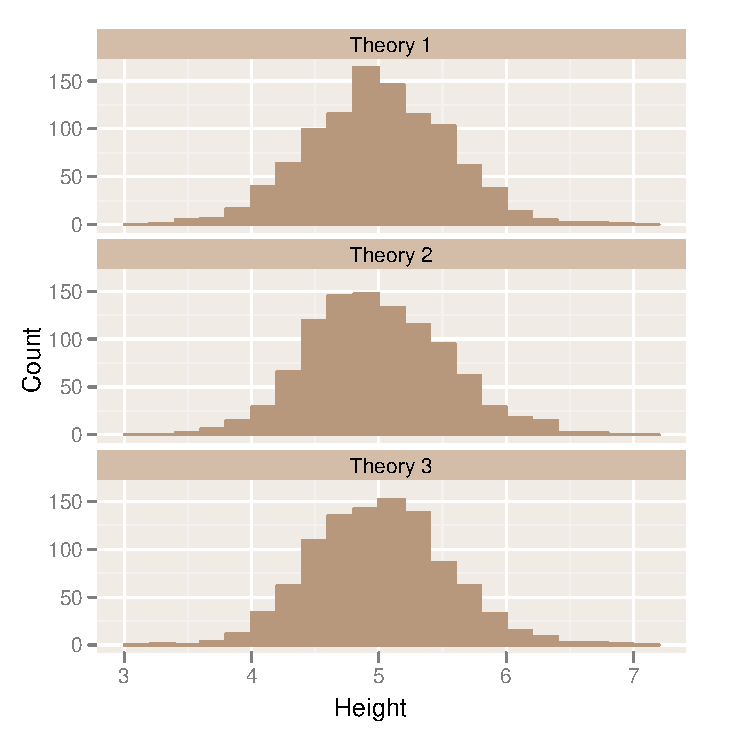
\includegraphics[width=12.5cm,height=12.5cm]{favir-graphs/p1.pdf}\caption{Prior Marginal Distributions}\label{prior}\end{center}\end{figure}
The R code above defined the initial parameters and samples 1000
heights from each prior marginal distribution.  These samples are then
used to plot a histogram shown in figure \ref{prior}.  As you can see,
the marginal distributions look somewhat similar.

\clearpage

\subsection{Example Data}

To continue the sample, we now sample the heights of 100 people.  The
results are shown in figure \ref{height samples}.  This is the
evidence we will use to compare the three theories.

\begin{figure}[htp] \normalsize 
\begin{center}
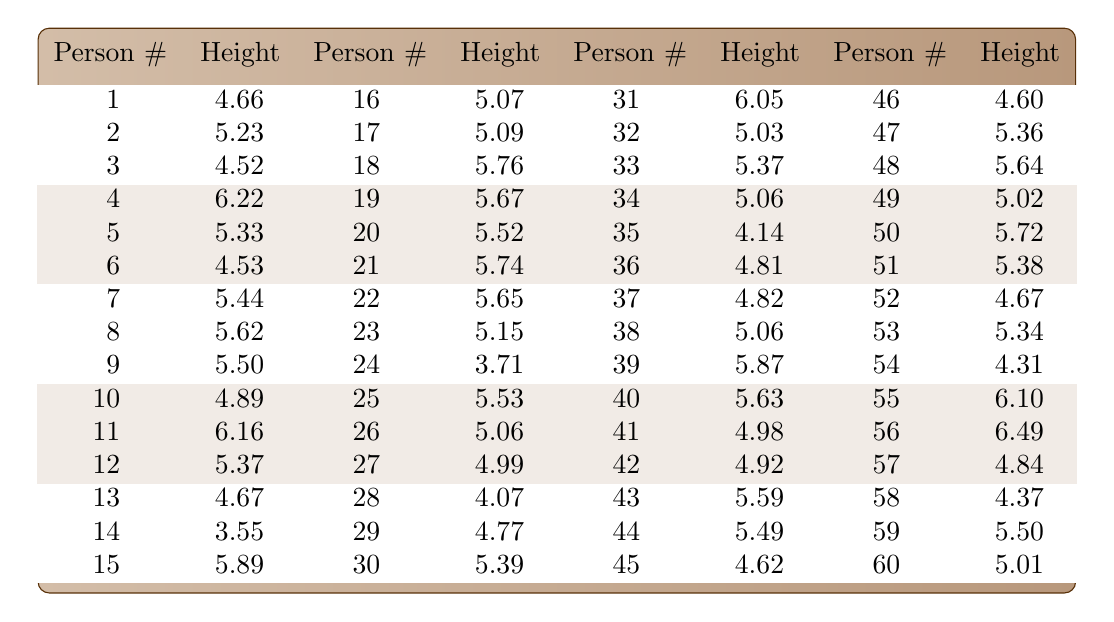
\begin{tikzpicture}
\node (tbl) {
\begin{tabular} { D{!}{!}{2.0}D{!}{!}{4.0}D{!}{!}{2.0}D{!}{!}{4.0}D{!}{!}{2.0}D{!}{!}{4.0}D{!}{!}{2.0}D{!}{!}{4.0} }  
\multicolumn{1}{c}{Person \#} & \multicolumn{1}{c}{Height} & \multicolumn{1}{c}{Person \#} & \multicolumn{1}{c}{Height} & \multicolumn{1}{c}{Person \#} & \multicolumn{1}{c}{Height} & \multicolumn{1}{c}{Person \#} & \multicolumn{1}{c}{Height} \\
 \addlinespace 
\rowcolor{white}
$1$ & $4.66$ & $16$ & $5.07$ & $31$ & $6.05$ & $46$ & $4.60$\\

\rowcolor{white}
$2$ & $5.23$ & $17$ & $5.09$ & $32$ & $5.03$ & $47$ & $5.36$\\

\rowcolor{white}
$3$ & $4.52$ & $18$ & $5.76$ & $33$ & $5.37$ & $48$ & $5.64$\\

\rowcolor{colorM1}
$4$ & $6.22$ & $19$ & $5.67$ & $34$ & $5.06$ & $49$ & $5.02$\\

\rowcolor{colorM1}
$5$ & $5.33$ & $20$ & $5.52$ & $35$ & $4.14$ & $50$ & $5.72$\\

\rowcolor{colorM1}
$6$ & $4.53$ & $21$ & $5.74$ & $36$ & $4.81$ & $51$ & $5.38$\\

\rowcolor{white}
$7$ & $5.44$ & $22$ & $5.65$ & $37$ & $4.82$ & $52$ & $4.67$\\

\rowcolor{white}
$8$ & $5.62$ & $23$ & $5.15$ & $38$ & $5.06$ & $53$ & $5.34$\\

\rowcolor{white}
$9$ & $5.50$ & $24$ & $3.71$ & $39$ & $5.87$ & $54$ & $4.31$\\

\rowcolor{colorM1}
$10$ & $4.89$ & $25$ & $5.53$ & $40$ & $5.63$ & $55$ & $6.10$\\

\rowcolor{colorM1}
$11$ & $6.16$ & $26$ & $5.06$ & $41$ & $4.98$ & $56$ & $6.49$\\

\rowcolor{colorM1}
$12$ & $5.37$ & $27$ & $4.99$ & $42$ & $4.92$ & $57$ & $4.84$\\

\rowcolor{white}
$13$ & $4.67$ & $28$ & $4.07$ & $43$ & $5.59$ & $58$ & $4.37$\\

\rowcolor{white}
$14$ & $3.55$ & $29$ & $4.77$ & $44$ & $5.49$ & $59$ & $5.50$\\

\rowcolor{white}
$15$ & $5.89$ & $30$ & $5.39$ & $45$ & $4.62$ & $60$ & $5.01$  \end{tabular}};
\begin{pgfonlayer}{background}
\draw[rounded corners,left color=colorM2,right color=colorM3,draw=colorM5]
    ($(tbl.north west)+(0.14,0.00)$) rectangle
           ($(tbl.south east)-(0.14,0.00)$);
\end{pgfonlayer}
\end{tikzpicture} \caption{Sampled Heights} \label{height samples} \end{center}\end{figure}
\section{Sampling From the Posterior}

The next step is to sample from the posterior of each distribution's
parameters.  1000 samples will be taken from each posterior
distribution.

This is somewhat trivial for theories 1 and 2 because they are
Bayesian conjugates.  In fact, the marginal likelihood is analytically
soluable so there is no need to use the \texttt{margLikArrogance}
package.  They were chosen as an example so the output of the package
can be compared to the exact answer.  The code that computes them is
shown below.

\begin{Schunk}
\begin{Sinput}
> UpdateMean <- function(mean.mean, mean.sd, sd, x) {
+     post.sd <- sqrt(1/(1/mean.sd^2 + length(x)/sd^2))
+     return(c(mean = (mean.mean/mean.sd^2 + sum(x)/sd^2) * post.sd^2, 
+         sd = post.sd))
+ }
> set.seed(1)
> t1.post.param <- UpdateMean(t1.mean.mean, t1.mean.sd, t1.sd, 
+     samples)
> t1.post.samples <- rnorm(1000, mean = t1.post.param["mean"], 
+     sd = t1.post.param["sd"])
> t2.post.param <- UpdateMean(t2.mu.mean, t2.mu.sd, t2.sigma, log(samples))
> t2.post.samples <- rnorm(1000, mean = t2.post.param["mean"], 
+     sd = t2.post.param["sd"])
\end{Sinput}
\end{Schunk}

For theory 3 we will sample from the posterior by taking advantage of
the semi-conjugacy of our model and coding a Gibbs sampler.  The code
is shown below.

\begin{Schunk}
\begin{Sinput}
> UpdatePrecision <- function(prec.shape, prec.rate, mean, x) {
+     return(c(shape = prec.shape + length(x)/2, rate = prec.rate + 
+         sum((x - mean)^2)/2))
+ }
> t3.mean.post.samples <- rep(NA, 1010)
> t3.sd.post.samples <- rep(NA, 1010)
> t3.mean.post.samples[1] <- 5
> t3.sd.post.samples[1] <- 0.5
> set.seed(1)
> for (i in 2:1010) {
+     mu.params <- UpdateMean(t3.mean.mean, t3.mean.sd, t3.sd.post.samples[i - 
+         1], samples)
+     t3.mean.post.samples[i] <- rnorm(1, mu.params["mean"], mu.params["sd"])
+     prec.params <- UpdatePrecision(t3.prec.shape, t3.prec.rate, 
+         t3.mean.post.samples[i - 1], samples)
+     t3.sd.post.samples[i] <- sqrt(1/rgamma(1, shape = prec.params["shape"], 
+         rate = prec.params["rate"]))
+ }
> t3.post.samples <- cbind(t3.mean.post.samples, t3.sd.post.samples)[11:1010, 
+     ]
> colnames(t3.post.samples) <- c("mean", "sd")
\end{Sinput}
\end{Schunk}

\noindent This chain should be checked for tuning, convergence, etc.,
but here we will just assume we have obtained the posterior samples we
wanted.  The prior and posterior parameter distributions are shown in
figure \ref{parameter comparison}.

\begin{figure}\begin{center}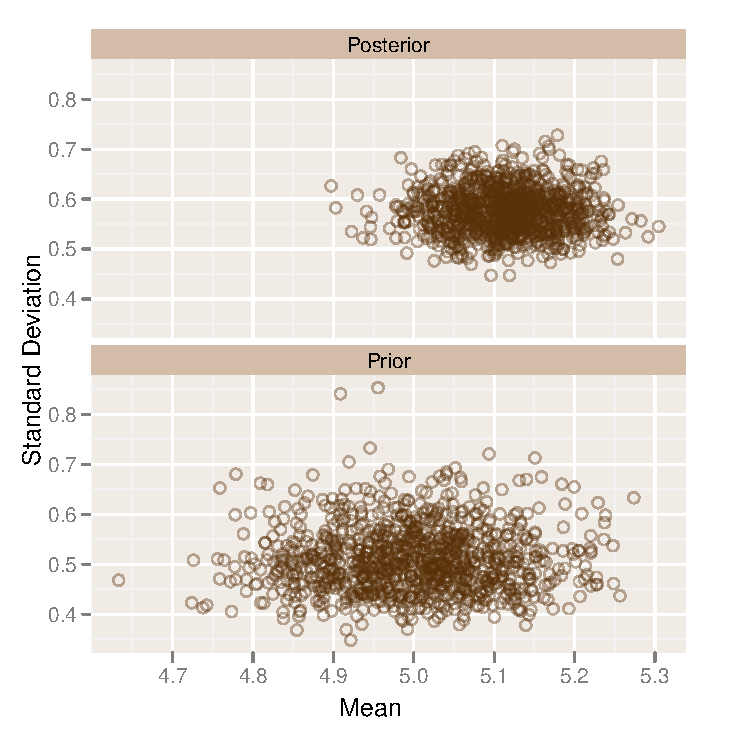
\includegraphics[width=12.5cm,height=12.5cm]{favir-graphs/pcomp_plot.pdf}\caption{Theory 3 Prior vs Posterior Parameters}\label{parameter comparison}\end{center}\end{figure}
\subsection{Sampled Likelihoods}

We have the sampled posterio parameter distributions for each theory;
the next step is compute the value $\mbox{log}\,p(\bx \wedge
\btheta_{j,i} | T_i) = \mbox{log}(p(\bx | \btheta_{j,i},
T_i)p(\btheta_{j,i}|T_i))$ for each point $\btheta_{j,i}$.  For theory
1 we have:

\begin{Schunk}
\begin{Sinput}
> T1OneLik <- function(theta) {
+     ll <- sum(dnorm(samples, mean = theta, sd = t1.sd, log = TRUE))
+     return(ll + dnorm(theta, mean = t1.mean.mean, sd = t1.mean.sd, 
+         log = TRUE))
+ }
> t1.ll <- sapply(t1.post.samples, T1OneLik)
\end{Sinput}
\end{Schunk}

\noindent For theory 2:

\begin{Schunk}
\begin{Sinput}
> T2OneLik <- function(theta) {
+     ll <- sum(dlnorm(samples, meanlog = theta, sdlog = t2.sigma, 
+         log = TRUE))
+     return(ll + dnorm(theta, mean = t2.mu.mean, sd = t2.mu.sd, 
+         log = TRUE))
+ }
> t2.ll <- sapply(t2.post.samples, T2OneLik)
\end{Sinput}
\end{Schunk}

\noindent Finally, for theory 3 we have:

\begin{Schunk}
\begin{Sinput}
> T3OneLik <- function(theta) {
+     ll <- sum(dnorm(samples, mean = theta[1], sd = theta[2], 
+         log = TRUE))
+     param.ll <- (dnorm(theta[1], mean = t3.mean.mean, sd = t3.mean.sd, 
+         log = TRUE) + dgamma(1/theta[2]^2, shape = t3.prec.shape, 
+         rate = t3.prec.rate, log = TRUE))
+     return(ll + param.ll)
+ }
> t3.ll <- apply(t3.post.samples, 1, T3OneLik)
\end{Sinput}
\end{Schunk}

\section{Using the Package and Comparing the Theories}
\label{Compute}

We can now apply the \texttt{margLikArrogance} package to compute each
theory's marginal likelihood.  The following are the only three lines
in this example that actually use the package!

\begin{Schunk}
\begin{Sinput}
> library(margLikArrogance)
> t1.margll <- MarginalLikelihood(matrix(t1.post.samples, ncol = 1), 
+     t1.ll)
> t2.margll <- MarginalLikelihood(matrix(t2.post.samples, ncol = 1), 
+     t2.ll)
> t3.margll <- MarginalLikelihood(t3.post.samples, t3.ll, bounds = matrix(c(-Inf, 
+     Inf, 0.1, Inf), nrow = 2))
\end{Sinput}
\end{Schunk}

\noindent The results are summarized in figure \ref{results}.  The
posterior probability shown assumes that each theory had probability
one-third before the data was observed.  Note that the \texttt{bounds}
argument was used for theory 3, specifying that the standard deviation
cannot be negative.

\begin{figure}[htp] \normalsize 
\begin{center}
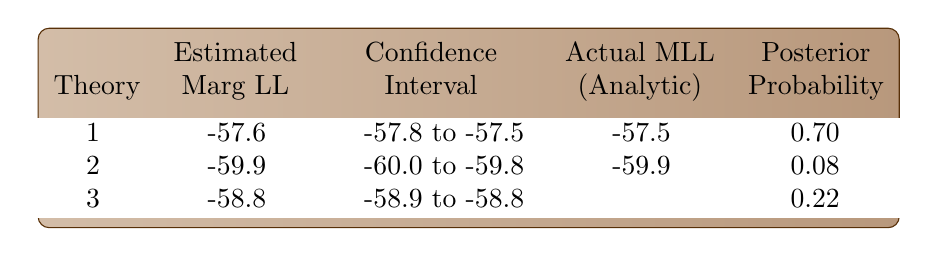
\begin{tikzpicture}
\node (tbl) {
\begin{tabular} { D{!}{!}{1.0}D{!}{!}{5.0}D{!}{!}{14.0}D{!}{!}{5.0}D{!}{!}{4.0} }  
\multicolumn{1}{c}{} & \multicolumn{1}{c}{Estimated} & \multicolumn{1}{c}{Confidence} & \multicolumn{1}{c}{Actual MLL} & \multicolumn{1}{c}{Posterior}\\

\multicolumn{1}{c}{Theory} & \multicolumn{1}{c}{Marg LL} & \multicolumn{1}{c}{Interval} & \multicolumn{1}{c}{(Analytic)} & \multicolumn{1}{c}{Probability} \\
 \addlinespace 
\rowcolor{white}
$1$ & $-57.6$ & $-57.8 to -57.5$ & $-57.5$ & $0.70$\\

\rowcolor{white}
$2$ & $-59.9$ & $-60.0 to -59.8$ & $-59.9$ & $0.08$\\

\rowcolor{white}
$3$ & $-58.8$ & $-58.9 to -58.8$ & $$ & $0.22$  \end{tabular}};
\begin{pgfonlayer}{background}
\draw[rounded corners,left color=colorM2,right color=colorM3,draw=colorM5]
    ($(tbl.north west)+(0.14,0.00)$) rectangle
           ($(tbl.south east)-(0.14,0.00)$);
\end{pgfonlayer}
\end{tikzpicture} \caption{Arrogance Sampling Results} \label{results} \end{center}\end{figure}
\subsection{Qualitative Comparisons}

Instead of computing posterior probabilities directly, we can
reference the table from Kass and Raftery (figure \ref{guidelines})
when interpreting the results in figure \ref{results}.  According to
that, the sample data is positive evidence for theory 1 versus theory
3.  The data does not help us much to decide between theories 1 and 3
or theories 2 and 3.

\begin{figure}[htp] \normalsize 
\begin{center}
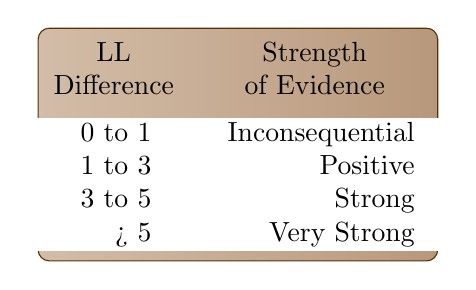
\begin{tikzpicture}
\node (tbl) {
\begin{tabular} { D{!}{!}{6.0}D{!}{!}{15.0} }  
\multicolumn{1}{c}{LL} & \multicolumn{1}{c}{Strength}\\

\multicolumn{1}{c}{Difference} & \multicolumn{1}{c}{of Evidence} \\
 \addlinespace 
\rowcolor{white}
$0 to 1$ & $Inconsequential$\\

\rowcolor{white}
$1 to 3$ & $       Positive$\\

\rowcolor{white}
$3 to 5$ & $         Strong$\\

\rowcolor{white}
$   > 5$ & $    Very Strong$  \end{tabular}};
\begin{pgfonlayer}{background}
\draw[rounded corners,left color=colorM2,right color=colorM3,draw=colorM5]
    ($(tbl.north west)+(0.14,0.00)$) rectangle
           ($(tbl.south east)-(0.14,0.00)$);
\end{pgfonlayer}
\end{tikzpicture} \caption{Kass and Raftery's Guidelines} \label{guidelines} \end{center}\end{figure}

\section{A More Challenging Example}

The \texttt{margLikArrogance} package requires samples $\btheta_{j,i}$
from the posterior parameter distribution $\btheta_i|\bx,T_i$ and the
value of $\mbox{log}\, p(\bx \wedge \btheta_{j,i}|T_i)$ at each point.
Because 

\[ p(\btheta_i|\bx, T_i) = \frac{p(\bx \wedge \btheta_i| T_i)}{p(\bx|T_i)},\]

\noindent computing the marginal likelihood $p(\bx,T_i)$ is equivalent
to computing the normalizing constant for an unknown density
$p(\btheta_i|\bx,T_i)$, given samples from $\btheta_i|\bx,T_i$ and the
unnormalized density $p(\bx \wedge \btheta_i| T_i)$ at each point.

Thus we can test the algorithm by suppling samples from an arbitrary
density along with densities multiplied by an arbitrary constant.  In
this section, we try the algorithm on a 50/50 mixture of two
15-dimensional normal distributions.  The first has mean at
\[ \mu_1 = (1, 0, 0, 0, 0, 0, 0, 0, 0, 0, 0, 0, 0, 0, 0). \]
The second has mean at $\mu_2 = 10^6 \mu_1$.  Both will have the
identity covariance matrix.  The code below generates $n = 100000$
samples from this distribution are generated below.

\begin{Schunk}
\begin{Sinput}
> library(mvtnorm)
> mvn.n <- 10^5
> mvn.mu1 <- c(1, rep(0, 14))
> mvn.mu2 <- 10^6 * mvn.mu1
> set.seed(1)
> mvn.theta <- rbind(rmvnorm(mvn.n/2, mean = mvn.mu1), rmvnorm(mvn.n/2, 
+     mean = mvn.mu2))
\end{Sinput}
\end{Schunk}

The log likelihood of the samples are computed below.  An arbitrary
constant 1000 is added to each log-likelihood (equivalent to scaling
each likelihood by a factor of $e^{1000}$).  This means that the
correct marginal log-likelihood is 1000.

\begin{Schunk}
\begin{Sinput}
> mvn.ll <- (1000 + log(dmvnorm(mvn.theta, mean = mvn.mu1)/2 + 
+     dmvnorm(mvn.theta, mean = mvn.mu2)/2))
\end{Sinput}
\end{Schunk}

We can then apply the algorithm the same way as in section
\ref{Compute}.

\begin{Schunk}
\begin{Sinput}
> mvn.mll <- MarginalLikelihood(mvn.theta, mvn.ll)
> mvn.mll$mll
\end{Sinput}
\begin{Soutput}
[1] 1000.626
\end{Soutput}
\begin{Sinput}
> mvn.mll$conf.interval
\end{Sinput}
\begin{Soutput}
[1] 1000.380 1000.953
\end{Soutput}
\end{Schunk}

The algorithm returns a reasonable approximation of the correct
log-likelihood 1000, and has a reasonably small confidence interval.

\section{Conclusion}

In this vignette we have applied the \texttt{margLikArrogance} package
to two example problems.  The first was detailed and involved choosing
between three models of people's height distributions.  The second was
abstract but quick, and involved a bimodal 15-dimensional posterior
parameter distribution.  In applications such as these, I hope the
\texttt{margLikArrogance} package can provide an easy and useful way
to approximate marginal likelihoods.


\end{document}
